%\documentclass[11pt,a4paper,uplatex,dvipdfmx]{ujarticle} 		% for uplatex
\documentclass[11pt,a4j,dvipdfmx]{jarticle} 					% for platex
\input{pieces/form00_header} % pieces
\input{pieces/kakenhi7} % pieces
% form01_header.tex
% 2017-05-28 Split from form00_header.tex to move \input{kakenhiLaTeX7.sty} to mother_1.tex.
% 2010-01-15 Adjusted margins.
% ===== Parameters for KL (Kakenhi LaTeX) ========================
%%\geometry{noheadfoot,scale=1}  %scale=1 resets margins to 0
\setlength{\unitlength}{1pt}

\newlength{\KLCella}
\newlength{\KLCellb}
\newlength{\KLCellc}
\newlength{\KLCelld}
\newlength{\KLCelle}
\newlength{\KLCellf}

\newcounter{KLMaxYearCount}	% # of years for the proposal
\newcommand{\KLCLLang}{}	% language-dependent left-justification in tabular

% ===== format and header =========
% 2020-01-15: Reset it to match the margins (25 mm on sides, 20 mm on top and bottom). 
% A4: 294 mm x 210 mm.  
% LaTeX's default margin is 1 inch = 25.4 mm.
\setlength{\oddsidemargin}{-1pt}	% (25.0 - 25.4) / 25.4 * 72 pt/inch = -1 pt
\setlength{\evensidemargin}{-1pt}
\setlength{\textwidth}{453pt}		% (210 - 25*2) / 25.4 * 72 = 453 pt
\setlength{\topmargin}{-61pt}	% This and \headheight determine the actual top margin
\setlength{\textheight}{254mm}		% (294 - 20*2) = 254 mm

\setlength{\headheight}{48pt}
\setlength{\headsep}{3pt}

\cfoot{}
\renewcommand{\headrulewidth}{0pt}

\pagestyle{empty}
% ==== other applications table =========
\newcommand{\KLTableHeaderFont}{\fontsize{8.2}{11}\selectfont}
\newcommand{\KLTableHeaderSmallFont}{\fontsize{7.5}{10}\selectfont}
\newcommand{\KLTableHeaderSmallerFont}{\fontsize{7}{10}\selectfont}

 % pieces
% ===== Global year-dependent definitions for the Kakenhi form ===========
% 基本情報
\newcommand{\研究開始年度}{2022}
\newcommand{\研究開始元号年度}{04}	%令和

\newcommand{\一年目西暦}{2022}
\newcommand{\二年目西暦}{2023}
\newcommand{\三年目西暦}{2024}
\newcommand{\四年目西暦}{2025}
\newcommand{\五年目西暦}{2026}
\newcommand{\六年目西暦}{2027}

\newcommand{\一年目}{4}
\newcommand{\二年目}{5}
\newcommand{\三年目}{6}
\newcommand{\四年目}{7}
\newcommand{\五年目}{8}
\newcommand{\六年目}{9}

\newcommand{\一年目J}{4}
\newcommand{\二年目J}{5}
\newcommand{\三年目J}{6}
\newcommand{\四年目J}{7}
\newcommand{\五年目J}{8}
\newcommand{\六年目J}{9}


 % pieces
\input{pieces/hook3} % pieces
%#Name: kiban_s
% form04_jsps_headers.tex
% 2017-08-20 Taku
% 2017-08-29 Taku
%			Added a check against jsps-abs-p1-header.
% 2017-09-02 Taku
%			Added sectionNo to the commands to make them compatible with 
%			\KLBeginSubjectWithHeaderCommands.
%			Use \KLJInt.
% 2018-09-01 Taku
%			Adjusted the heights of the headers by inserting \vspace{-3pt} and \rule.
%
\newcommand{\headerfont}{\fontsize{11}{11}\selectfont}
% ===== Headers =====================================
\newcommand{\JSPSVeryFirstPageStyle}[5]{%
%	Defines the header for the very first page of the form.
%	Called from \KLShumokuFirstPageStyle in form04_***.
%--------------------------------
%	#1: page style name
%	#2: 様式
%	#3: 研究種目名
%	#4: 項目名
%	#5: sectionNo
%--------------------------------
	\fancypagestyle{JSPSVeryFirstPageStyle}{% The name is not taken from #1, because 
		\fancyhf{}
		\fancyhead[L]{\hspace{-37pt}\headerfont#2\ 研究計画調書(添付ファイル項目)\\
				\rule{0pt}{18pt}\\}
%				\rule{0pt}{0pt}\\}
		\fancyhead[R]{\headerfont\textbf{#3\ \KLJInt{\thepage}}\vspace{-5pt}\\
			\rule{0pt}{0pt}\\}
%		\fancyhead[R]{\headerfont\textbf{#3\ \KLJInt{\thepage}\\}}
	}
	\thispagestyle{JSPSVeryFirstPageStyle}
}

\newcommand{\JSPSFirstSubjectPageStyle}[5]{%
%	Defines the header for the first page for the subject.
%	Called from \KLShumokuFirstPageStyle in form04_***.
%--------------------------------
%	#1: page style name
%	#2: 様式
%	#3: 研究種目名
%	#4: 項目名
%	#5: sectionNo
%--------------------------------
	\fancypagestyle{JSPSFirstSubjectPageStyle}{%
		\fancyhf{}
		\fancyhead[R]{\headerfont\textbf{#3\ \KLJInt{\thepage}}\vspace{-5pt}\\
			\rule{0pt}{0pt}\\}
%		\fancyhead[R]{\headerfont\textbf{#3\ \KLJInt{\thepage}\\}}
	}
	\thispagestyle{JSPSFirstSubjectPageStyle}
}

\newcommand{\JSPSDefaultPageStyle}[5]{%
%	Defines the default header for the subject.
%	Called from \KLShumokuDefaultPageStyle in form04_***.
%--------------------------------
%	#1: page style name
%	#2: 様式
%	#3: 研究種目名
%	#4: 項目名
%	#5: sectionNo
%--------------------------------
	\fancypagestyle{JSPSDefaultPageStyle}{%
		\fancyhf{}
		\fancyhead[L]{\headerfont\textbf{【#4(つづき)\ 】}\vspace{-7pt}\\}
		\fancyhead[R]{\headerfont\textbf{#3\ \KLJInt{\thepage}}\vspace{-5pt}\\
			\rule{0pt}{0pt}\\}
%		\fancyhead[R]{\headerfont\textbf{#3\ \KLJInt{\thepage}\\}}	
        }
        \pagestyle{JSPSDefaultPageStyle}
}

 % pieces
% form04_kiban_s_header.tex
% 2018-09-02 Taku: Revised headers for JFY2019 style with (sub page#).

\usepackage{watermark}

% ===== Global definitions for the Kakenhi form ======================
% 基本情報
\newcommand{\様式}{Form S-11:}
\newcommand{\研究種目}{Scientific Research}
\newcommand{\研究種目後半}{}
\newcommand{\研究種別}{ (S)}
\newcommand{\研究種目header}{\研究種目\研究種別\研究種目後半}

\newcommand{\KLMainFile}{kiban\_s.tex}
\newcommand{\KLYoshiki}{kiban_s_header}

% ===== Headers =====================================
\fancypagestyle{kiban-s-pub-subject-header}{%
	\fancyhf{}
	\fancyhead[L]{\framebox{\headerfont\parbox{0.65\textwidth}{To be filled in and attached to the Research Proposal Document for\\ each Principal Investigator (PI) and Co-Investigator(s) (Co-I(s))}}\\}
	\fancyhead[R]{\headerfont\textbf{\研究種目\研究種別\ 9-(\thepage)\\}}
}

\fancypagestyle{kiban-s-pub-header}{%
	\fancyhf{}
	\fancyhead[L]{\headerfont\textbf{[4. Proposal of the Researcher (PI) (continued from the previous page)]}}
	\fancyhead[R]{\headerfont\textbf{\研究種目\研究種別\ 9-(\thepage)\\}}
}

%==== specific commands for kiban_s ================
\newcommand{\研究者氏名}{}
\newcommand{\研究者氏名ふりがな}{}
\newcommand{\研究者生年月日の年}{}
\newcommand{\研究者生年月日の月}{}
\newcommand{\研究者生年月日の日}{}
\newcommand{\研究者年齢}{}
\newcommand{\研究者所属機関部局職}{}
\newcommand{\研究者学位}{}

\newcommand{\KLXi}{}
\newcommand{\KLYi}{}
\newcommand{\KLYii}{}
%============================================
 % pieces
% ===== Global definitions for the Kakenhi form ======================
% 基本情報
%
%------ 研究課題名  -------------------------------------------
\newcommand{\研究課題名}{象の卵}

%----- 研究機関名と研究代表者の氏名-----------------------
\newcommand{\研究機関名}{逢坂大学}
\newcommand{\研究代表者氏名}{湯川秀樹}
\newcommand{\me}{\underline{\underline{H.~Yukawa}}} 
%---- 研究期間の最終年度 ----------------
\newcommand{\研究期間の最終元号年度}{8}  %令和で、半角数字のみ
%========================================

% inst_general.tex
%--------------------------------------------------------------------
% For writing instructions
%--------------------------------------------------------------------
\newcommand{\KLInstWOGeneral}[1]{%
	\noindent
 ーー Note ーーーーーーーーーーーーーーーーーーーーーーーーーーーーーー\\
		#1\\
 ーーーーーーーーーーーーーーーーーーーーーーーーーーーーーーーーーーーーーーーー
}

\newcommand{\KLInst}[1]{%
	\noindent
	\ifthenelse{\equal{#1}{}}{%
 ーー Note ーーーーーーーーーーーーーーーーーーーーーーーーーーーーーーー\\
	}{%
 ーー Note\textcircled{1} ーーーーーーーーーーーーーーーーーーーーーーーーーーーーーーー\\
		#1\\
		
	\noindent
 ーー Note\textcircled{2} ーーーーーーーーーーーーーーーーーーーーーーーーーーーーーーー\\
	}
}

\newcommand{\KLInstLine}[1]{%
	\ifthenelse{\equal{#1}{}}{%
 ーー Note ーーーーーーーーーーーーーーーーーーーーーーーーーーーーーー\\
	}{%
 ーー Note\textcircled{#1} ーーーーーーーーーーーーーーーーーーーーーーーーーーーーーーー\\
	}
}

\newcommand{\KLInstructionTitle}{%
	\textbf{\large Matters to be noted when preparing the Research Proposal Document}\\
}

\newcommand{\DeleteInstructions}[1]{%
	\textcolor{red}{Read the following important notes carefully before preparing this form. Delete this entire text box when filling in this form.\\
 (Delete \texttt{\textbackslash #1} and other text)}%
}

% local variables for \GeneralInstructions ------------------------
\newcommand{\留意事項内種目名}{}			% #1
\newcommand{\留意事項内記入要領名}{}		% #2
\newcommand{\留意事項内種目名削除用}{}	% #3

\newcommand{\KakenhiInstructions}{%
    \textbf{1.以下の内容を熟読・理解の上、研究計画調書を作成すること。\\
  ーーーーーーーーーーーーーーーーーーーーーーーーーーーーーーーーーーーーーーーーーーー\\
    \begin{small}
     科研費は、研究者の自由な発想に基づく全ての分野にわたる研究を格段に発展させることを目的とし、\\
    豊かな社会発展の基盤となる独創的・先駆的な研究を支援します。\\
     科研費では、応募者が自ら自由に課題設定を行うため、提案課題の学術的意義に加え、独自性や創造性\\
    が重要な評価ポイントになります。このため、「基盤研究」及び「若手研究」の研究計画調書様式では、\\
    学術の潮流や新たな展開などどのような「学術的背景」の下でどのような「学術的『問い』」を設定した\\
    か、当該課題の「学術的独自性や創造性」、「着想に至った経緯」、「国内外の研究動向と本研究の位置\\
    付け」はどのようなものか、などの記述を求めています。\\
     審査においては、総合審査又は二段階書面審査における審査委員間の議論・意見交換等により研究課題\\
    の核心を掴み、学術的な意義や独自性、創造性など学術的重要性を評価するとともに、実行可能性並びに\\
    研究遂行能力も含めて総合的に判断します。\\
     科研費に応募するに当たっては、上記に留意の上、公募要領や審査基準、様式の説明書き等を十分に確\\
    認し、審査委員に学術的重要性等が適切に伝わるように研究計画調書を作成してください。\\
    \end{small}%
  ーーーーーーーーーーーーーーーーーーーーーーーーーーーーーーーーーーーーーーーーーーー\\
    }
}

\newcommand{\GeneralInstructions}[3]{%
	\ifthenelse{\equal{#1}{}}{%
		\renewcommand{\留意事項内種目名}{研究計画調書}%
	}{%
		\renewcommand{\留意事項内種目名}{#1}%
	}%
	\ifthenelse{\equal{#2}{}}{%
		\renewcommand{\留意事項内記入要領名}{作成・記入要領}%
	}{%
		\renewcommand{\留意事項内記入要領名}{#2}%
	}%
	\ifthenelse{\equal{#3}{}}{%
		\renewcommand{\留意事項内種目名削除用}{\留意事項内種目名}%
	}{%
		\renewcommand{\留意事項内種目名削除用}{#3}%
	}%
	1. Read carefully the ``Procedures for Preparing and Entering a Research Proposal Document'' when preparing the document.\\
	2. The document should be written with font size 10-point or larger.\\
	3. The title and instructions on the upper part of each page should be left intact.\\
	4. Do not exceed the maximum number of pages specified in the instructions. In case blank page(s) occur, leave them as they are (do not eliminate any page).\\ 
 \DeleteInstructions{JSPSInstructions}\\
 ーーーーーーーーーーーーーーーーーーーーーーーーーーーーーーーーーーーーーーーー
}


\newcommand{\PapersInstructions}{%
 ーー Note ーーーーーーーーーーーーーーーーーーーーーーーーーーーーーーー\\
\begin{small}%
 1. 研究業績(論文、著書、産業財産権、招待講演等)は、網羅的に記載するのではなく、本研\\
   究計画の実行可能性を説明する上で、その根拠となる文献等の主要なものを適宜記載するこ\\
   と。\\
 2.研究業績の記述に当たっては、当該研究業績を同定するに十分な情報を記載すること。\\
   例として、学術論文の場合は論文名、著者名、掲載誌名、巻号や頁等、発表年(西暦)、著\\
   書の場合はその書誌情報、など。\\
 3.論文は、既に掲載されているもの又は掲載が確定しているものに限って記載すること。\\
 \DeleteInstructions{PapersInstructions}\\
\end{small}
 ーーーーーーーーーーーーーーーーーーーーーーーーーーーーーーーーーーーーーーーー\\
} % pieces
%inst_kiban_s.tex
\newcommand{\JSPSInstructions}{%
	\\
	\KLInstLine{}
	\KLInstructionTitle
	\DeleteInstructions{JSPSInstructions}\\
	\KLInstLine{1}
	\KakenhiInstructions

	\noindent
	\KLInstLine{2}
  1.基盤研究(S)は審査区分表の大区分により、広い分野の委員構成で多角的視点から総合\\
    審査が行われることに留意の上、研究計画調書を作成すること。\\

	\noindent
	\KLInstLine{3}
	\GeneralInstructions{}{}{}
}

\newcommand{\JSPSInstructionsB}{%
	\KLInstWOGeneral{%
  ※ 研究組織が研究代表者のみで構成される場合には、「(3)研究組織全体の研究環\\
    境」の記述は不要です。\\
  \DeleteInstructions{JSPSInstructionsB}
	}
}
 % pieces
% user07_header
% ===== my favorite packages ====================================
% ここに、自分の使いたいパッケージを宣言して下さい。
\usepackage{wrapfig}
%\usepackage{amssymb}
%\usepackage{mb}
%\DeclareGraphicsRule{.tif}{png}{.png}{`convert #1 `dirname #1`/`basename #1 .tif`.png}
\usepackage{lineno}

% ===== my personal definitions ==================================
% ここに、自分のよく使う記号などを定義して下さい。
\newcommand{\klpionn}{K_L \to \pi^0 \nu \overline{\nu}}
\newcommand{\kppipnn}{K^+ \to \pi^+ \nu \overline{\nu}}

% ----- 業績リスト用 -------------
\newcommand{\paper}[6]{%
	% paper{title}{authors}{journal}{vol}{pages}{year}
	\item ``#1'', #2, #3 {\bf #4}, #5 (#6).			% お好みに合わせて変えてください。
}

\newcommand{\etal}{\textit{et al.\ }}
\newcommand{\ca}[1]{*#1}	% corresponding author;   \ca{\yukawa}  みたいにして使う
\newcommand{\invitedtalk}{招待講演}

\newcommand{\yukawa}{H.~Yukawa}					% no underline
%\newcommand{\yukawa}{\underline{\underline{H.~Yukawa}}}	% with 2 underlines
\newcommand{\tomonaga}{S.~Tomonaga}

\newcommand{\prl}{Phys.\ Rev.\ Lett.\ }		% よく使う雑誌も定義すると楽

% ===== 欄外メモ ==================
\newcommand{\memo}[1]{\marginpar{#1}}
%\renewcommand{\memo}[1]{}	% 全てのメモを表示させないようにするには、行頭の"%"を消す


%\input{../../sample/simple/contents}	% skip
\input{pieces/hook5} % pieces

\begin{document}
\input{pieces/hook7} % pieces
%#Split: 01_purpose_plan  
%#PieceName: p01_purpose_plan
% p01_purpose_plan_00.tex
\KLBeginSubject{01}{1}{1. Research Objectives, Research Method, etc.}{5}{F}{}{jsps-p1-header}{jsps-default-header}

\section{1 研究目的、研究方法など}
%    <<最大 6ページ>>

%s02_purpose_plan_with_abstract
\noindent
\textbf{(概要)}\\
%begin 研究目的及び研究計画の概要空行付き ====================
本研究の目的は、象の卵を発見して、象の卵生を証明することである。
進化論的には、象は卵を産む方が自然である。

	世界の動物園や、アフリカ、インドで
	空と陸の両面から多角的に探索を行う。
	象の卵を発見した場合は、
	その形状の測定、材質の解析、工学的応用の可能性の検討を行う。
\vspace*{7zw} % (概要)と(本文)の間が10行程度になるよう、必要に応じて値を調整してください。
	
%end 研究目的及び研究計画の概要空行付き ====================

\noindent
\rule{\linewidth}{1pt}\\
\noindent
\textbf{(本文)}
%begin 研究目的と研究計画	====================
\JSPSInstructions	% <-- 留意事項。これは消すか、コメントアウトしてください。

\textbf{\\     *** 以下は、あくまで例です。真似しないでください。 ***\\
     *** 本文はもちろん、節の切り方や論理の組み方は   ***\\
     *** ご自分の気に入ったスタイルで書いてください。  ***}

\subsection{なぜ象は卵を産むはずか}
今まで、哺乳類である象は卵を産まないとされてきた。
しかし、哺乳類の定義は乳を与える動物のことであり、
必ずしも胎盤を持ち母親の体内で成長させる動物であるとは限らない。
たとえばカモノハシは卵を産むし、カンガルーは体外の袋の中で新生児を育てる。
哺乳類の動物が胎生か卵胎生か卵生かは、進化上の分類よりもむしろ、生活の環境によって決まる。
象のように大きく強い動物の場合、重たい象の胎児を運ぶよりは、
卵を産んでその重さから解放される方が楽である。
また卵が大きく硬い殻でできていれば、他の動物に取られたり食べられたりする恐れもない。
さらに食物を求めて象の群れが移動するときも、長い鼻で丸い卵を転がして行った方が、
胎児を持ち運ぶよりエネルギー効率が高い。
(恐竜も卵を産んだが、長い鼻を持たず、車輪を考案するだけの脳を持たなかったため、巣を作った)
こうした点から、象は卵を産む方が進化論的に自然である。

\subsection{象など大型哺乳類の卵は今まで見つかってないのか}
寺村輝夫の研究\cite{teramura}によれば、昔、
王子の誕生を祝って国民全員に卵焼きを提供すべく、
軍隊を動員して象の卵を探させた王がいた。
このときは孵化直後の子象は見つかったが、それが入っていた殻の発見には至っていない。

また、私は今まで地球上で最大の哺乳類であるシロナガスクジラの卵の探索を行ってきた。
まだ発見には至っていないが、海水単位体積あたりの存在確率の上限値を与えた(私の業績リストの中の[\ref{pub:whale}])。

\subsection{今こそ、枠を越えた自由な発想を}
今まで、我々研究者は分野や古い学説など様々な枠にとらわれてきた。
しかし今や、科研費の書類では全体を囲む枠が取り払われたのみならず、
研究目的、背景、方法などの間の枠も取り除かれた。
これにより我々研究者は、自分の主張を、細切れにされることなく、
自分の論理的な道筋に従って書類に書ける自由を得た。
しかし逆に言えば、一目で数ページの中のどこに何が書いてあるのかがわかる
文章を書くことが重要である。
そのためには、論文など論理的な文章を書くときに使い慣れた\LaTeX を用いるのが楽である。

書類の枠から解放された今、\framebox{象=胎生}という\underline{常識の枠}からも我々は解放され、
より\textbf{自由な発想}をするべきである。

\textbf{ん??この研究の目的が何か、どこでも言ってないぞ。。。}

\subsection{どうやって探すか}
予算と時間は限られているため、確率と効率を考慮し、
次のような順序で象の卵を探索する。
\begin{enumerate}
	\item 逢坂北部のある終点駅の駅前では、
            	毎年年末になると図\ref{fig:egg_R}、図\ref{fig:egg_L}に示すように
            	コンクリートでできた象の卵の像のまわりを電飾するしきたりが残っている。
            	(少し寄り目にし、右目で左の図、左目で右の図を見てください。
            	なお、このように図や表を横に並べる方が、{\tt wrapfigure}を用いるより位置の調整が楽です。)
		まずは超音波を使い、このコンクリートの内側に化石化した象の卵が実は隠されていないか、
		調査する。
                \begin{figure}[h]
                 	\begin{minipage}[t]{0.49\linewidth}
            			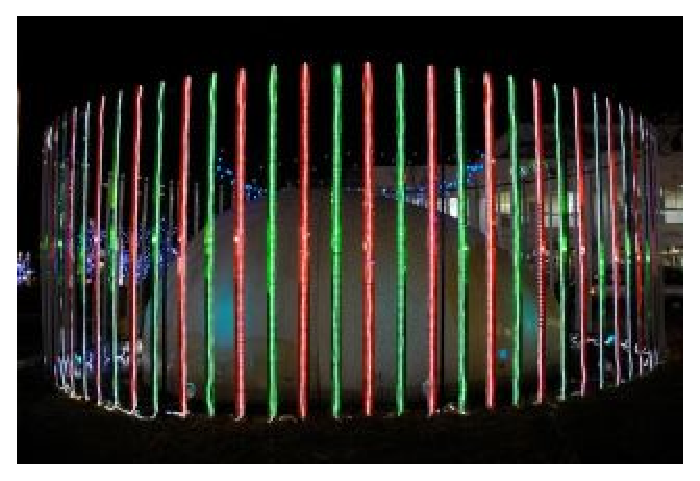
\includegraphics[width=\linewidth]{figs/egg_R.eps}
            			\caption{右目用}
            			\label{fig:egg_R}
                		\end{minipage}
                		\hspace{0.01\linewidth}
                		\begin{minipage}[t]{0.49\linewidth}
            			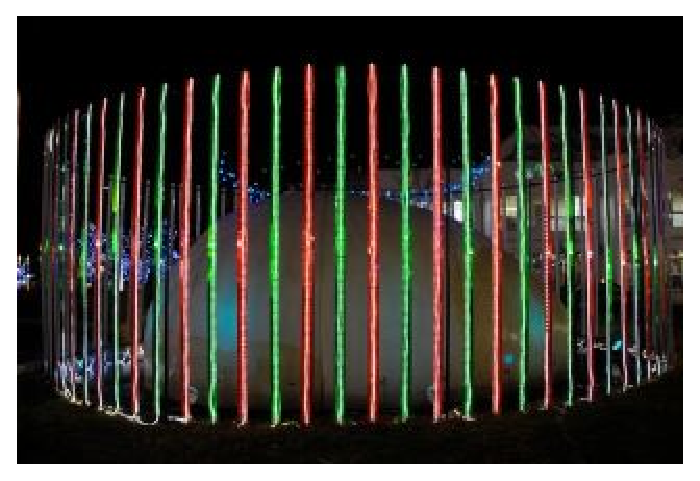
\includegraphics[width=\linewidth]{figs/egg_L.eps}
            			\caption{左目用}
            			\label{fig:egg_L}
        			\end{minipage}
                 \end{figure}
                 
	\item 世界の動物園を巡り、
            	象舍の藁の山の中に卵が隠されていないか、探す。
		これは藁の山の中から針を探すより楽である。

	\item 見通しの効くアフリカのサバンナで、宇宙と地上から象の卵を探す。
		定期的に撮った写真を比較する、超新星探索と同じ画像処理を衛星写真に対して行えば、
		効率的に広範囲の探索ができる。
		象の卵の候補が見つかったら、ハッブル望遠鏡をその方向に向けて写真を撮り、
		現地調査に向かうべきかどうかを判定する。

	\item インドとタイに行き、ジャングルに隠されている卵を探す。
                	ジャングルの場合空からは探しにくいが、象使いも多く、象の背中に乗って
                	象の視点から探索することができる。
                	さらに、気性の荒いアフリカ象と異なり、気だての優しいインド象ならば
                	卵の在処を教えてくれる可能性もある。
		子供時代、象と散歩をした経験があるので\cite{inTheForest}、
		すぐに象と仲良くなれると思う。
		
\end{enumerate}

\subsection{この研究の売り}
本研究は次のような特徴を持つ。
\begin{itemize}
	\item 象が卵を産むなどという考えは\textbf{創造的}(想象的)である。
	\item 象の卵を探索しようとする研究は現在世界中で他になく、\textbf{独創的}である。
		従って私がこの分野の第一人者(一人者:ひとりもの?)である。
	\item 身近すぎてつい見逃しがちな箇所の探索、最新の映像や画像技術を駆使した探索、
		象の優しさを活用した探索など、多方面からの探索である。
\end{itemize}

\subsection{象の卵を発見したら}
         \begin{wrapfigure}{r}{5cm}
         		\begin{center}
		         
\includegraphics[width=5cm]{figs/seagull2.eps}
		         \caption{カモメ}
		         \label{fig:seagull}
	         \end{center}
         \end{wrapfigure}
象の卵を発見したら、次のことを行う。
\subsubsection{外形の計測}
        外形を計測し、それが
        \framebox{絶対的な卵の形の枠}である
        アルキメデス(\('A\rho\chi i\mu\acute{\eta}\delta\eta\mbox{\c{c}}\))の
        円筒座標表示形(式(\ref{eq:archimedes}))と一致するかどうか調べる。
        もし一致していなければ、卵でない可能性がある。
        \begin{equation}
        	\label{eq:archimedes}
        	r(z) = 0.5\sqrt{1-(e^z-2)^2}
        \end{equation}

\subsubsection{殻の化学構造の解明}
	殻の化学的構造を解析し、その強さの秘密を解明する。
	象の卵の殻は、80kgを超える体重の子象と、
	その栄養源である卵黄の大きな質量を支えるだけではなく、
	卵を暖める親の象の体重も支える必要がある。
	このため、象の卵の殻は、体重の軽い鳥類(図\ref{fig:seagull})の卵の殻とは
	本質的に異なる構造を持っていると考えられる。
	化学的構造が解明できれば、それを人工的に合成して新たな自動車や飛行機の
	ボディに利用できる。

	%blahblah
An elephant was born from a big egg.
That big egg was hatched by its mother elephant.
That mother elephant was born from another egg.
That big egg was hatched by its mother elephant.
That mother elephant was born from another egg.
That big egg was hatched by its mother elephant.
That mother elephant was born from another egg.
That big egg was hatched by its mother elephant.
That mother elephant was born from another egg.
That big egg was hatched by its mother elephant.
That mother elephant was born from another egg.
That big egg was hatched by its mother elephant.
That mother elephant was born from another egg.
That big egg was hatched by its mother elephant.
That mother elephant was born from another egg.
That big egg was hatched by its mother elephant.
That mother elephant was born from another egg.
That big egg was hatched by its mother elephant.
That mother elephant was born from another egg.
That big egg was hatched by its mother elephant.
That mother elephant was born from another egg.
That big egg was hatched by its mother elephant.
That mother elephant was born from another egg.
That big egg was hatched by its mother elephant.
That mother elephant was born from another egg.
That big egg was hatched by its mother elephant.
That mother elephant was born from another egg.
That big egg was hatched by its mother elephant.
That mother elephant was born from another egg.
That big egg was hatched by its mother elephant.
That mother elephant was born from another egg.
That big egg was hatched by its mother elephant.
That mother elephant was born from another egg.
That big egg was hatched by its mother elephant.
That mother elephant was born from another egg.
That big egg was hatched by its mother elephant.
That mother elephant was born from another egg.
That big egg was hatched by its mother elephant.
That mother elephant was born from another egg.
That big egg was hatched by its mother elephant.
That mother elephant was born from another egg.
That big egg was hatched by its mother elephant.
That mother elephant was born from another egg.
That big egg was hatched by its mother elephant.
That mother elephant was born from another egg.
That big egg was hatched by its mother elephant.
That mother elephant was born from another egg.
That big egg was hatched by its mother elephant.
That mother elephant was born from another egg.
That big egg was hatched by its mother elephant.
That mother elephant was born from another egg.
That big egg was hatched by its mother elephant.
That mother elephant was born from another egg.
That big egg was hatched by its mother elephant.
That mother elephant was born from another egg.
That big egg was hatched by its mother elephant.
That mother elephant was born from another egg.
That big egg was hatched by its mother elephant.
That mother elephant was born from another egg.
That big egg was hatched by its mother elephant.
That mother elephant was born from another egg.
That big egg was hatched by its mother elephant.
That mother elephant was born from another egg.
That big egg was hatched by its mother elephant.
That mother elephant was born from another egg.
That big egg was hatched by its mother elephant.
That mother elephant was born from another egg.
That big egg was hatched by its mother elephant.
That mother elephant was born from another egg.
That big egg was hatched by its mother elephant.
  % << only for demonstration. Please delete it or comment it out.
	%blahblah
An elephant was born from a big egg.
That big egg was hatched by its mother elephant.
That mother elephant was born from another egg.
That big egg was hatched by its mother elephant.
That mother elephant was born from another egg.
That big egg was hatched by its mother elephant.
That mother elephant was born from another egg.
That big egg was hatched by its mother elephant.
That mother elephant was born from another egg.
That big egg was hatched by its mother elephant.
That mother elephant was born from another egg.
That big egg was hatched by its mother elephant.
That mother elephant was born from another egg.
That big egg was hatched by its mother elephant.
That mother elephant was born from another egg.
That big egg was hatched by its mother elephant.
That mother elephant was born from another egg.
That big egg was hatched by its mother elephant.
That mother elephant was born from another egg.
That big egg was hatched by its mother elephant.
That mother elephant was born from another egg.
That big egg was hatched by its mother elephant.
That mother elephant was born from another egg.
That big egg was hatched by its mother elephant.
That mother elephant was born from another egg.
That big egg was hatched by its mother elephant.
That mother elephant was born from another egg.
That big egg was hatched by its mother elephant.
That mother elephant was born from another egg.
That big egg was hatched by its mother elephant.
That mother elephant was born from another egg.
That big egg was hatched by its mother elephant.
That mother elephant was born from another egg.
That big egg was hatched by its mother elephant.
That mother elephant was born from another egg.
That big egg was hatched by its mother elephant.
That mother elephant was born from another egg.
That big egg was hatched by its mother elephant.
That mother elephant was born from another egg.
That big egg was hatched by its mother elephant.
That mother elephant was born from another egg.
That big egg was hatched by its mother elephant.
That mother elephant was born from another egg.
That big egg was hatched by its mother elephant.
That mother elephant was born from another egg.
That big egg was hatched by its mother elephant.
That mother elephant was born from another egg.
That big egg was hatched by its mother elephant.
That mother elephant was born from another egg.
That big egg was hatched by its mother elephant.
That mother elephant was born from another egg.
That big egg was hatched by its mother elephant.
That mother elephant was born from another egg.
That big egg was hatched by its mother elephant.
That mother elephant was born from another egg.
That big egg was hatched by its mother elephant.
That mother elephant was born from another egg.
That big egg was hatched by its mother elephant.
That mother elephant was born from another egg.
That big egg was hatched by its mother elephant.
That mother elephant was born from another egg.
That big egg was hatched by its mother elephant.
That mother elephant was born from another egg.
That big egg was hatched by its mother elephant.
That mother elephant was born from another egg.
That big egg was hatched by its mother elephant.
That mother elephant was born from another egg.
That big egg was hatched by its mother elephant.
That mother elephant was born from another egg.
That big egg was hatched by its mother elephant.
  % << only for demonstration. Please delete it or comment it out.
		

\vspace*{1zw}
\begin{thebibliography}{99}
	\bibitem{teramura} 寺村輝夫、「ぼくは王様 - ぞうのたまごのたまごやき」.
	\bibitem{inTheForest} マリー・ホール・エッツ、「もりのなか」.
\end{thebibliography}
%end 研究目的と研究計画	====================

% p01_purpose_plan_01.tex
\KLEndSubject{F}


%#Split: 02_rights  
%#PieceName: p02_rights
% p02_rights_00.tex
\KLBeginSubject{02}{2}{2. Issues Relevant to Human Right Protection and Legal Compliance}{1}{F}{}{jsps-subject-header}{jsps-default-header}

\section{2 人権の保護及び法令等の遵守への対応}
%    <<最大 1ページ>>

% s09_rights
%begin 人権の保護及び法令等の遵守への対応 ====================
	象の卵のES細胞の培養、象のクローンの生成などは行わない。
	象個体を現地から持ち出すことはないので、ワシントン条約ならびに
        生物多様性条約に抵触しない。また、組換え実験は行なわないので、
        カルタヘナ議定書にも抵触しない。

        \noindent
        \rule{\linewidth}{1pt}
        \linenumbers
        \subsection{ついでに\LaTeX の便利な機能}
        \subsubsection{節}
        通常通り\textbackslash subsection, \textbackslash subsubsectionなどが使えます。
        番号は自動的につきます。
        
        \subsubsection*{番号なし節}
        \textbackslash subsubsection* のように* 付きを使うと、節の番号がつきません。
        
        \subsubsection{コメント文}
        %う〜ん、これ言おうか言わまいか迷てんねんけどな、
        %言うのも何やし、言わへんのもどうかと思うし、どうしようかなあ....
        \LaTeX では当たり前ですが、
        今はとりあえず消すけど使う可能性のある文章は、
        消さずに行の頭に \% をつけてコメントアウトすると、後で復活できます。
        \texttt{TeXShop}や\texttt{TeXWorks}では、複数行選んでまとめてコメントにしたり
        コメントから外したりできます。
        
        \subsubsection{編集用の行番号}
        \texttt{lineno}というパッケージを使えば、
        \textbackslash linenumbersと\textbackslash nolinenumbersの間の行に行番号が振られます。
        これは編集中に他の人からコメントをもらうときに便利です。\\
        \textbf{最終版のPDFを作る前に、行番号は消してください。}
        
        \subsubsection{編集用の欄外のメモ}
        \textbackslash memo{}を使うと右の例のように、欄外にメモを書けます。\\
        \memo{欄外メモ\\だよ}
        \textbf{最終版のPDFを作る前に、\LaTeX ソースファイルの60行目付近にある指示に従って、}
        \textbackslash memo \textbf{を無効化してください。}
        
        \nolinenumbers
%end 人権の保護及び法令等の遵守への対応 ====================

% p02_rights_01.tex
\KLEndSubject{F}


%#Split: 03_final_year  
%#PieceName: p03_final_year
% p03_final_year_00.tex
\KLBeginSubject{03}{3}{3 研究計画最終年度前年度応募を行う場合の記述事項}{1}{F}{}{jsps-subject-header}{jsps-default-header}

\section{3 研究計画最終年度前年度応募を行う場合の記述事項}
%    <<最大 1ページ>>

%s04_prep_finalyear
% 2020-08-16: Taku: Adjusted the horizontal position of the tabular.
%begin 最終年度の研究課題 ====================
\newcommand{\最終年度研究種目名}{基盤研究(Z)}
\newcommand{\最終年度研究課題番号}{99999}
\newcommand{\最終年度研究課題名}{シロナガスクジラの卵はなぜ見つけられないのか}
\newcommand{\最終年度研究期間}{平成25年度〜令和\一年目 年度}
%end 最終年度の研究課題 ====================
% p03_final_year_01.tex
\noindent
\hspace{-8pt}
\begin{tabular}{|p{118pt}|p{44pt}|p{208pt}|p{46pt}|}
	\hline
	\KLTabC{\textbf{研究種目名}} & 
	\KLTabC{\textbf{課題番号}} & 
	\KLTabC{\textbf{研究課題名}} & 
	\KLTabC{\textbf{研究期間}}\\
	\hline
	\最終年度研究種目名 &
	\最終年度研究課題番号 &
	\最終年度研究課題名 &
	\最終年度研究期間 \\
	\hline
\end{tabular}
\\


\noindent
\textbf{当初研究計画及び研究成果}\\
%begin 研究計画最終年度の応募の計画と成果 ====================
	研究課題の通り、シロナガスクジラの卵は見つけられなかった。
%end 研究計画最終年度の応募の計画と成果 ====================
\\

\noindent
\textbf{前年度応募する理由}\\
%begin 研究計画最終年度の応募の理由 ====================
	さっさと次の研究に移りたいので。
%end 研究計画最終年度の応募の理由 ====================

% p03_final_year_02.tex
\KLEndSubject{F}


%#Split: members_info % keep

% 研究代表者の調書 (not 長所) ===============
\KLInput{daihyo_info}

% 研究分担者の調書 ===============
\KLInput{buntansha_info}

% 研究分担者を追加する場合は、buntansha_info.tex を複製して別の名前にし、
% この下に追加してください。
% \input ではなく、\KLInput を用いると、読み込んだファイルの中で定義した
% マクロはそのファイルの中でのみ有効となり、他のファイルでの定義と干渉しません。
%\KLInput{taro_info}
%\KLInput{hanako_info}
%\KLInput{jiro_info}
%\KLInput{saburo_info}


%#Split: 99_tail
\input{pieces/hook9} % pieces
\end{document}

